\documentclass[14pt]{extarticle}
\usepackage[utf8]{inputenc}
\usepackage[T1]{fontenc}
\usepackage[spanish,es-lcroman]{babel}
\usepackage{amsmath}
\usepackage{amsthm}
\usepackage{physics}
\usepackage{tikz}
\usepackage{float}
\usepackage[autostyle,spanish=mexican]{csquotes}
\usepackage[per-mode=symbol]{siunitx}
\usepackage{gensymb}
\usepackage{multicol}
\usepackage{enumitem}
\usepackage[left=2.00cm, right=2.00cm, top=2.00cm, 
     bottom=2.00cm]{geometry}

%\renewcommand{\questionlabel}{\thequestion)}
\decimalpoint
\sisetup{bracket-numbers = false}

\title{\vspace*{-2cm} Indicaciones para presentar el examen parcial \\  Grupo 43 - Física III\vspace{-5ex}}
\date{}

\begin{document}
\maketitle

\large

A continuación se señala la organización y logística para presentar el primer examen parcial de Física III Grupo 43.

\begin{enumerate}
\item Cada alumno deberá de tener en la paleta de la silla: bolígrafo tinta negra o azul, lápiz, goma, borrador, sacapuntas y calculadora.
\item No se permite el uso de celular o tableta.
\item Toda mochila se dejará al frente del salón, debiendo guardar el celular en la mochila.
\item No se permitirá el préstamo de elementos, por ello deberán de llegar prevenidos.
\item No van a ocupar hojas adicionales, por lo que cuadernos, libretas, carpetas, no serán necesarias.
\item Todo el grupo deberá estar sentado en estricto orden alfabético minutos antes de las 11:50 am, comenzando en la primera fila del lado izquierdo, es decir, del lado de la puerta del salón. El alumno(a) con el número de lista 1, estará en la primera silla, el alumno(a) con el número de lista 2, en la segunda silla de la misma fila, hasta completar la última silla, el siguiente alumno(a) en la lista, tomará la primera silla de la siguiente fila y así sucesivamente.
\item Tendrán 50 minutos para resolver el examen: \textbf{\underline{inicia 11:50 am}} y termina \textbf{\underline{12:40 pm}}
\item El pase de lista se realizará mientras se entrega el examen a cada alumno.
\item No podrán retirarse del salón durante el examen.
\item La alumna/alumno que haya terminado el examen antes de que concluyan los 50 minutos, levantará la mano para que el Profesor se acerque y tome su examen, debiendo de permanecer en su banca. No podrán salir del salón, mantendrán el orden y permanecerán en silencio, no tomarán la mochila, menos encenderán su celular, dado que habrá estudiantes que continúan en el examen. Los alumnos que hayan entregado su examen \textbf{siguen bajo la instrucciones generales} y se les puede cancelar el examen: en caso de sospecha de que estén pasando información.
\item Se notificará al grupo cuando falten 5 minutos para acabar el tiempo del examen como aviso para que vayan preparando la entrega. A los dos minutos se recordará para que vayan concluyendo.
\item A las 12:40 pm el Profesor ya no recibirá algún examen, quien no lo entregue debidamene, se le considerará como examen no presentado.
\item Se anexa la carátula institucional del examen, para que revisen las indicaciones.
\begin{figure}[H]
    \centering
    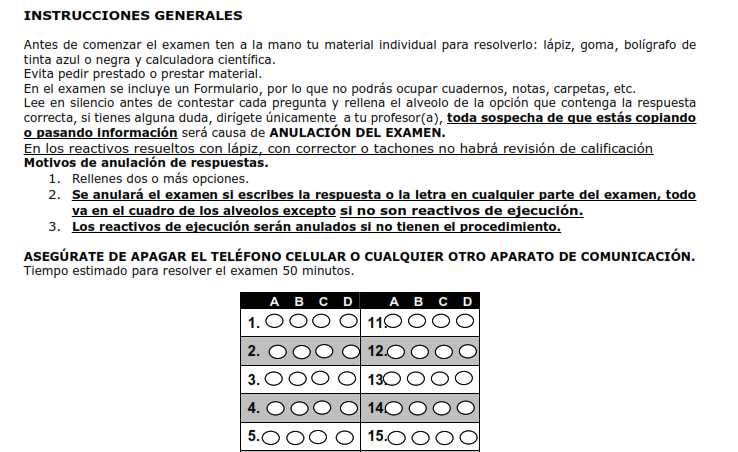
\includegraphics[scale=0.9]{Imagenes/Instrucciones_Examen.png}
\end{figure}
\item Recuerden que cuando se indique en el examen \textbf{Ejercicio de ejecución}, se requiere que anoten el procedimiento, desarrollo y solución en la hoja, identificando el número de problema que están resolviendo.
\item Si un \textbf{Ejercicio de ejecución} no incluye el desarrollo, no contabiliza en el puntaje así se haya seleccionado la respuesta correcta.
\item Para cualquier duda sobre las Instrucciones Generales, tienes la oportunidad hasta antes del día del examen, de enviarme un mensaje para resolver cualquier inquietud.
\end{enumerate}

\end{document}